%%% Laboratory	 Notes
%%% Template by Mikhail Klassen, April 2013
%%% Contributions from Sarah Mount, May 2014
\documentclass[a4paper]{tufte-handout}

\newcommand{\workingDate}{\textsc{Dec $|$ 2016}}
\newcommand{\userName}{Felix Engstr\"om}
\newcommand{\institution}{KTH}

\usepackage{lab_notes}

\usepackage{hyperref}
\hypersetup{
    pdffitwindow=false,            % window fit to page
    pdfstartview={Fit},            % fits width of page to window
    pdftitle={Projekt lab notes 2016},     % document title
    pdfauthor={Felix Engstr\"om},         % author name
    pdfsubject={},                 % document topic(s)
    pdfnewwindow=true,             % links in new window
    colorlinks=true,               % coloured links, not boxed
    linkcolor=DarkScarletRed,      % colour of internal links
    citecolor=DarkChameleon,       % colour of links to bibliography
    filecolor=DarkPlum,            % colour of file links
    urlcolor=DarkSkyBlue           % colour of external links
}


\title{Project lab notes}
\date{2016}

\begin{document}
\maketitle

%%%%%%%%%%%%%%%%%%%%%%%%%%%%%%%%%%%%%%%%%%%%%%%%%%%%%%%%

\begin{projects}
	\begin{description}
		\item Exploration and implementation of algorithm for classification of 
            signal-peptides.
    \end{description}
\end{projects}

%%%%%%%%%%%%%%%%%%%%%%%%%%%%%%%%%%%%%%%%%%%%%%%%%%%%%%%%
\newday{19 December 2016}

We have decided to mainly focus on implementing a classifier using some sort of HMM approach. 
If there is time we will also try to do something using an RNN. The first step will be writing code to handle and import the data.


\newday{20 December 2016}

Today we implemented the first attempt at using an HMM. We used the hidden states from the data to train two models. One on the positive data and one on the negative data. We then used these to score the data points in the test set, choosing the model that had the highest probability score. 

\begin{figure}
    \begin{center}
      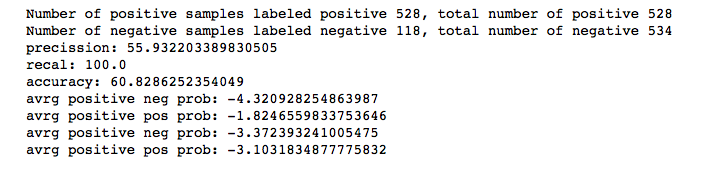
\includegraphics[width=0.8\textwidth]{pics/HMM_old.png}
    \end{center}
    \caption{Results from first run.}
\end{figure}

This approach did not fare so well. It seems that the mean probability of the negative model is much lower, creating a classifier that is overly prone to positive classification.

We will now try a different approach, were we instead train a model on all the samples, and have it predict a hidden state sequence for the given protein sequence. We then use the hidden state sequence to predict the class of the data by looking for "C".

I have also played around with an RNN but not quite fully grasped how to use it 

\begin{figure}
    \begin{center}
      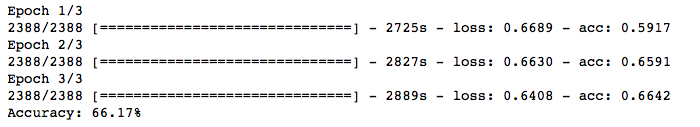
\includegraphics[width=0.8\textwidth]{./pics/first_run.png}
    \end{center}
    \caption{Results from first run.}
\end{figure}




\newday{21 December 2016}

Today we finished an single HMM approach to the problem. In this we use the
hidden-state data to create a markow model for all the peptides in the training
data. Then to classify new sequences we use the model to predict the the hidden
state of the sequence, and then look at the produced hiden-state to decide if
the sequence is a signal peptide. To decide if it is an signal peptide we simply look for a C in the state sequence.

\begin{figure}
    \begin{center}
      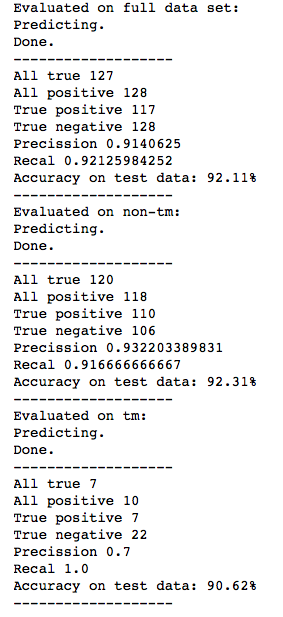
\includegraphics[width=0.3\textwidth]{pics/second_hmm_run.png}
    \end{center}
    \caption{Stats from the second run}
\end{figure}

\newday{22 December 2016}

We are now trying to use our model to analyze the proteome. We realized that
our model had no way of handling errors in the data, or '*' and had to adjust
for this. 

I also continued playing with the rnn. I have realized that the first attempt was implemented badly.
It would be interesting to try it but i would have to preprocess the data by first adding beginning and end of sentence markers and then concatenating all the sequences. I am still unclear of weather i should send the data in as onehot vectors or as integers. For now i will put this on ice. Concentrating on the hmm.

\newday{27 December 2016}
We have made some runs on the proteom and the result seems satisfactory

\begin{figure}
    \begin{center}
      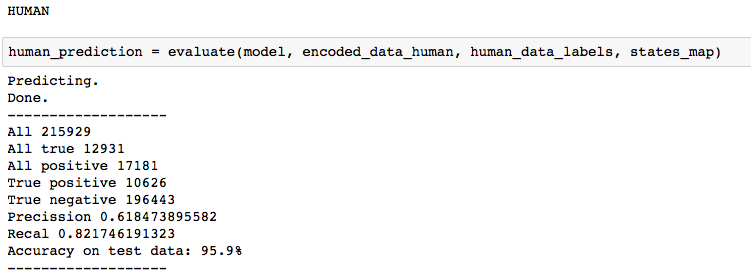
\includegraphics[width=0.8\textwidth]{pics/human_hmm_run.png}
    \end{center}
    \caption{Stats from the run on human and mouse proteom}

    \begin{center}
      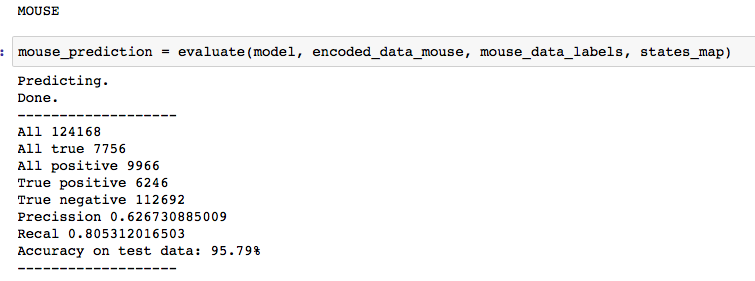
\includegraphics[width=0.8\textwidth]{pics/mouse_hmm_run.png}
    \end{center}
\end{figure}
\newday{28 december 2016}
Today we implemented controls for our experiment to ensure the validity of our results. We did this by generating random codon sequences of different length and assuming these should be negative and by adding noise at the end of positive and negative sequences. In these test we found that the classifier was overly prone to classify long random sequences as positive. Looking at the state sequences that the classifier created we identified that when the sequences were getting longer we were occasionally predicting "C" states in non signal peptide sequences of states. To adjust for this we changed the final step of the classifier to look for a valid sequence of states instead of just looking for a "C". This made accuracy on randomly created sequences of length 10,000 go from about 10 \% to about 90 \%. It also slightly improved the stats on the test data and proteoms. The other test did not find any anomalies.

\hrulefill

%%%%%%%%%%%%%%%%%%%%%%%%%%%%%%%%%%%%%%%%%%%%%%%%%%%%%%%%
\bibliographystyle{plain}
\bibliography{lab_notes}

\end{document}



